\documentclass[12pt, oneside, a4paper]{book}
%\usepackage{fullpage}
\usepackage[left=2.8cm,right=2.2cm,top=2 cm,bottom=2 cm]{geometry}
\usepackage{amsmath,amssymb}             % AMS Math
\usepackage[T1]{fontenc}
\usepackage[utf8]{inputenc}
\usepackage[french,english]{babel}
\usepackage{txfonts} 
\usepackage[]{graphicx}
\usepackage{multirow}
\usepackage{hyperref}

\renewcommand{\baselinestretch}{1.5}

\author{Aries Abdelkrime  \\[5 cm]
Encadreur : Zeggour Djamal Eddine \\
Co-encadreur: Hidouci Khaled Walid
}

\title{Vers une amélioration \\des résumés automatiques de textes}

\begin{document}

\selectlanguage {francais}
\pagestyle{empty} 

%\maketitle

\begin{center}
République Algérienne démocratique et populaire\\
Ministère de l'enseignement supérieur et de la recherche scientifique
\end{center}

\begin{center}
\noindent\rule{5 cm}{0.4pt}\\[2 cm]
\end{center}

\noindent
\begin{tabular}{ll}
\multirow{2}{*}{
\includegraphics[width=2cm]{img/esi-logo.png}} & \'Ecole national Supérieure d'Informatique\\
& \'Ecole doctorale STIC
\end{tabular}\\[2 cm]

\noindent
\begin{center}
{\LARGE \textbf{Vers une amélioration \\des résumés automatiques de textes}}\\[1 cm]
Rapport d'état d'avancement pour l'année 2013/2014.\\[3 cm]
\end{center}

\noindent
\begin{tabular}{lll}
Candidat& & ARIES Abdelkrime\\
Encadreur&& Pr. ZRGOUR Djamal Eddine \\
Co-encadreur && Pr. HIDOUCI Khaled Walid
\end{tabular}\\[2 cm]

\newpage

\pagestyle{plain}
\pagenumbering{arabic}


%============================================
%==== Description de notre problématique ====
%============================================
\chapter{Description de notre problématique}

\section{Introduction}

Avec l’augmentation considérable du volume des informations sur Internet, il est devenu très difficile de sélectionner l’information pertinente. 
L’information est publiée simultanément sur plusieurs canaux média avec des versions variantes, par exemple, un journal papier, un journal web, message SMS, des nouvelles de radio, etc. 
La personnalisation de l'information pour les différents canaux et formats est une fonction d'édition immense qui demande
notamment de raccourcir le texte original.
Le résumé automatique apporte une solution à ce problème et automatise complètement ce travail. 
En plus, les documents deviennent accessibles par d'autres langues en les résumant premièrement avant traduction, ceci peut être, dans la plupart des cas, suffisant pour juger de la pertinence d'un document avec une langue étrangère. 
De ce fait, on peut éviter le travail de traduction de tout le document manuellement.

D’après \cite{75-borko-bernier}, les résumés :
\begin{itemize}
\item Permettent d'économiser le temps de lecture, en fournissant l’essentiel de
l’information.
\item Facilitent la sélection (des livre qu’on veut lire, par exemple);
\item Facilitent les recherches documentaires;
\item Améliorent l'efficacité d'indexation. 
Le résumé automatique de textes joue un rôle très importants dans le développement de systèmes de recherche d'information efficaces et
performants \cite{03-allan-al}.
\end{itemize}

Voici quelques définitions:

\noindent
\textbf{Résumé automatique de textes:} C’est le processus qui réduit un document textuel au moyen de techniques informatiques, afin de créer une version condensée contenant les points les plus importantes dans le document original.

\noindent
\textbf{Recherche d’information (RI):} C’est le domaine qui étudie la manière de retrouver des informations pertinentes à un certain besoin à partir d’une collection de ressources d'information.

\noindent
\textbf{Traitement automatique du langage naturel (TALN):} C’est une discipline à la frontière de la linguistique, de l'informatique et de l'intelligence artificielle. 
Elle représente l’ensemble des recherches et développements visant à modéliser et reproduire, à l’aide de machines, la capacité humaine à produire et à comprendre des énoncés linguistiques dans des buts de communication.

\section{Problématique}

\subsection{Description}

La plupart des travaux dans le domaine du résumé automatique de textes sont basés sur l’approche par extraction \cite{58-luhn,69-edmundson}. 
Ils consistent à sélectionner les unités (phrases en général) censées être les plus pertinentes du texte source, et les concaténer pour avoir un résumé. 
Cette approche se base sur des critères de sélection (tf-idf, position, longueur, etc.) pour pondérer chaque unité déterminer celles qui sont pertinentes. 
Elle peut être indépendante de la langue et du genre du texte d’entrée et se caractérise par sa simplicité, mais elle soufre d’incohérence et parfois la redondance.
Par contre, l’approche par abstraction se base sur la reformulation du contenu du texte original, et la génération de nouvelles phrases, en se basant sur des techniques linguistiques. 
Cette approche fournit des résumés proches de celles des humains, mais dû à l’absence des outils TALN performants, cette approche est trop difficile.
Les techniques d’apprentissage sont souvent utilisées pour améliorer la tâche de résumé automatique \cite{05-yeh-al, 08-wong-al,10-yatsko-al}. 
L'objectif principal de tout algorithme d'apprentissage automatique est d'apprendre, d'identifier un ensemble de règles depuis un corpus de documents, ces règles sont ensuite appliquées sur le ou les textes en entrée du système de résumé. 
Le problème de cette technique est l’absence de corpus d’apprentissage libellés.

\subsection{Objectif}

L’objectif de ce travail est d’étudier les techniques de résumé automatique de textes, ainsi que les techniques de recherche d’information et ceux de traitement automatique de langage naturel applicables au domaine de résumé automatique. 
Ensuite, on veut utiliser ces techniques pour :
\begin{itemize}
\item Améliorer la solution proposée dans \cite{13-aries-al}.
\item Appliquer les techniques d’apprentissage pour améliorer le résumé résultant, en essayant de régler le problème d’absence des corpus étiquetés.
\item Appliquer les techniques linguistiques pour avoir des résumés plus précis.
\end{itemize}

Pour ce faire, nous avons opté du plan du travail suivant:
\begin{enumerate}
\item Etat de l’art \textbf{(12 mois)}
\item Proposition pour améliorer d’un premier papier \textbf{(12 mois)}
\item Validation avec deuxième papier \textbf{(16 mois)}
\item Rédaction de la thèse \textbf{(8 mois)}
\end{enumerate}


%============================================
%============= Etat de l'art ================
%============================================
\chapter{\'Etat de l'art}

Dans ce chapitre, nous allons présenter notre système considéré comme un système multilingue. 
Ensuite, on va parler sur d'autres systèmes récents. 
Enfin, nous allons discuter sur les problèmes qu'on peut faire face dans ce domaine.

\section{Notre système (All Summarizer)}

Pour éclairer notre état d'avancement, il faut d'abord présenter ce que nous avons déjà fait.
Avant de proposer notre méthode, nous avons fixé les buts suivant:
\begin{itemize}
\item Proposer une méthode qui est indépendante de la langue et du genre et domaine du document d'origine.
\item Cette méthode doit être rapide, et ne consomme pas les ressources mémoire.
\end{itemize}
Pour cette raison, nous avons utilisé des méthodes statistiques.
Si on choisi des critères comme la fréquences des termes dans le texte, la position de la phrase, sa longueur, etc., on peut attribuer à chaque phrase un score de pertinence pour chaque critère.
La méthode de calcule de score d'une phrase $P$ est donnée par l'équation \ref{eq:score-stat}. 
\begin{equation}
\label{eq:score-stat}
Score(P) = \sum_{1 \leq i \leq k} {\alpha_i * C_i(P)}
\end{equation}
Où:
\begin{itemize}
\item $k$ étant le nombre total de critères retenus pour calculer le score d'une phrase;
\item $C_i$ est la fonction calculant la valeur numérique d'un critère $ i $ appliqué à une phrase;
\item $\alpha_i$ est le coefficient associé au critère $ i $.
\end{itemize}

Pour fixer les poids de chaque critère, nous avant besoin d'un corpus pour faire l'apprentissage.
Mais, le problème qui se pose dans l'utilisation d'un corpus, est la dépendance à la langue et le genre du corpus.
Donc, il fallait penser à une autre solution qui estime les poids automatiquement, ou qui fusionne les scores d'une autre façon.
\begin{itemize}
\item On sait qu'un document contient plusieurs sujets (thèmes).
\item Les phrases similaires représentent, en général, le même sujet.
\item Un résumé est supposé être capable de représenter tous, ou la majorité des, sujets.
\end{itemize}
Notre proposition \cite{13-aries-al}, était de:

\noindent
Regrouper les phrases similaires dans des clusters, en utilisant la similarité cosinus et un seuil de regroupement $ th $.
Ici, l'équation \ref{eq:cosine-g} est utilisé pour calculer la similarité Cosinus entre deux phrases $ X $ et $ Y $.
\begin{equation}
\label{eq:cosine-g}
cos(X,Y) = \frac {\sum_i {x_i.y_i} }
{\sqrt{\sum_i(x_i)^2} . \sqrt{\sum_i(y_i)^2}}
\end{equation}
Où: $ x_i $ est le mot numéro $ i $ dans la phrase $ X $, et $ y_i $ est le mot numéro $ i $ dans la phrase $ Y $.

\noindent
Calculer la probabilité qu'une phrase représente tous les clusters (sujets) sachant un groupe de critères.
Ceci peut être représenté par l'équation suivante: 
\begin{equation}
\label{eq:sent-score}
P(s_i \in \bigcap_{j} C_j | \overrightarrow{f}) = 
\prod_{j} P(s_i \in C_j | \overrightarrow{f})
\end{equation}
Où $s_i$ est la phrase numéro $i$, $C_j$ est la classe $j$, et $\overrightarrow{f}$ est le vecteur de critères (fréquence de mots, longueur de phrase, position de phrase, etc.).
Après plusieurs simplifications, l'équation \ref{eq:sent-score} va être écrite comme suit:
\begin{equation}
\label{eq:class-score}
Score(s_i , \bigcap_{j} C_j , \overrightarrow{f}) = 
\prod_{j} \prod_{k} Score(s_i , C_j , f_k )
\end{equation}
Où:
\begin{equation}
\label{eq:score}
Score(s , C , f ) = 1 + \sum_{\phi \in s} {P(f=\phi | s \in C)}
\end{equation}
Et:
\begin{equation}
\label{eq:likelihood}
P(f = \phi | C) = \frac {F_{C\phi}}{\sum_{\phi'}{F_{C\phi'}}}
\end{equation}
$\phi$ est l'observation de le critère $ f $ dans la classe $ C $. 
$F_{C\phi}$ est le nombre d'apparition de $\phi$ dans la classe $ C $.


Le système (All Summarizer) est open-source (Apache-v2) et téléchargeable à partir de \url{https://github.com/kariminf/AllSummarizer}.


\section{Quelques systèmes multilingues}

Clustering has been used for summarization in many systems, either using documents as units, sentences or words. 
The resulted clusters are used to extract the summary.
Some systems use just the biggest cluster to score sentences and get the top ones. 
Others take from each cluster a representative sentence, in order to cover all topics. 
While there are systems, like ours, which score sentences according to all clusters.

``CIST" \cite{11-liu-al,13-li-al} is a system which uses hierarchical Latent Dirichlet Allocation topic (hLDA) model to cluster sentences into sub-topics.
A sub-topic containing more sentences is more important and therefore those containing just one or two sentences can be neglected.
The sentences are scored using hLDA model combined with some traditional features. 
The system participated for multi-document summarization task, where all documents of the same topic are merged into a big text document.

Likewise, ``UoEssex" \cite{11-elhaj-al} uses a clustering method (K-Means) to regroup similar sentences.
The biggest cluster is used to extract the summary, while other clusters are ignored. 
Then, the sentences are scored using their cosine similarities to the cluster's centroid. 
The use of the biggest cluster is justified by the assumption that a single cluster will give a coherent summary.

The scoring functions of these two systems are based on statistical features like frequencies of words, cosine similarity, etc.
In the contrary, systems like those of \cite{11-conroy-al} (``CLASSY"), \cite{11-varma-al} (``SIEL\_IIITH"), \cite{13-elhaj-rayson}, etc. are corpus-based summarizers, which can make it hard to introduce new languages.
``CLASSY" uses na\"ive Bayes to estimate the probability that a term may be included in the summary. 
The classifier was trained on DUC 2005-2007 data. 
As for backgrounds of each language, Wikinews are used to compute Dunning G-statistic.
``SIEL\_IIITH" uses a probabilistic Hyperspace Analogue to Language model. 
Given a word, it estimates the probability of observing another word with it in a window of size K, using a sufficiently large corpus. 
\cite{13-elhaj-rayson} calculate the log-likelihood of each word using a corpus of words frequencies and the multiLing'13 dataset. 
The score of each sentence is the sum of its words' log-likelihoods.



%============================================
%========== Notre contribution ==============
%============================================
\chapter{Notre contribution}

\chapter{Conclusion et perspectives}


\begin{itemize}

\item Régler le problème de choix pour le seuil de regroupement, ainsi que les critères utilisées. 
Pour ce faire, il faut entrainer deux réseaux de neurones: un spésifique pour l'estimation de seuil de regroupement, et l'autre pour décider est-ce qu'une critère d'extraction (TFU, TFB, POS, etc.) est bonne pour un document donné.

\item Tester notre système dans le contexte de résumé automatique multi-documents et multi-lingue, par rapport aux autres systèmes.

\item Trouver un moyen pour représenter les phrases et les relations entre eux, dans le but de reformuler le résumé extrait et produire un autre qui est plus lisible.

\end{itemize}



%Bibliographie
\bibliographystyle{ESIbib}
\bibliography{cite}

%\section{Estimation de seuil de regroupement}
%Puisque nous utilisons le seuil de regroupement ($ th $) avec les similarités entre les phrases pour décider quelles sont les phrases similaires, donc il y a une possibilité qu'on peut calculer ($ th $) à partir de ces similarités. 
%Pour ce faire, nous avons pensé d'utiliser des mesures statistiques sur ces similarités, donc nous avons utilisé les mesures suivants:
%\begin{itemize}
%\item La moyenne arithmétique des similarités;
%\item La variance des similarités;
%\item Le mode
%\item La médiane 
%\end{itemize}
%
%Donc, on veut trouver un modèle qu'on peut utiliser pour estimer le seuil à partir de ces 4 mesures. 
%Il est trop difficile de trouver un tel modèle, pour cette raison il faut utiliser l'apprentissage automatique.
%D'abord, il faut trouver des documents avec leurs résumés modèles.
%Pour chaque document, on calcul les 4 mesures concernant les similarités entre ces phrases et on choisi la valeur idéale de $ th $. 
%
%\section{L'apprentissage du seuil de regroupement}
%
%Les réseaux de neurone ont la capacité de prendre des valeurs en entrée et pondérer leurs poids afin de calculer la valeur souhaitée. Ils peuvent, aussi, générer des valeurs entre 0 et 1 en utilisant la fonction d'activation sigmoid: $ y = \frac{1}{1 + e^{-z}}  $ où $ z = b + \sum_{1}^{n} w_i x_i $. Ceci (la sortie) peut être considéré comme notre seuil de regroupement.
%
%La figure suivante représente un réseau de neuron qui a une couche d'entrée avec $ n $ noeuds, $ k-1 $ couches cachées avec ($ m $, ..., $ j $) noeuds et une couche de sortie avec $ k $ noeuds.
%Dans le reste du rapport, un réseaux comme ceci va représenté comme ça: \textbf{nxmx...xjxk}.
%
%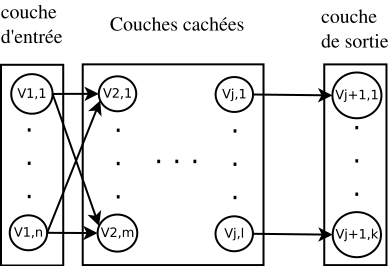
\includegraphics[width=15cm]{neural.pdf}
%
%\section{La préparation des données d'apprentissage}
%
%Nous avons utilisé le corpus \textbf{Cmplg} (181 documents) pour générer des résumés comme suite:
%\begin{itemize}
%\item Pour chaque combinaison des 5 critères: tf-unigrams, tf-bigrams, position, taille-réelle, taille-après-pretraitement (31 combinaisons)
%\begin{itemize}
%\item Pour chaque seuil de regroupement allant de 0 jusqu'à 1 avec un pas de 0.01 (101 seuils)
%\begin{itemize}
%\item Pour chaque document des 181 documents
%\begin{itemize}
%\item Générer un résumé
%\end{itemize}
%\end{itemize}
%\end{itemize}
%\end{itemize}
%Donc, nous avons générer 566711 résumés. 
%Pour ces résumés, nous avons observé que la plupart des résultats restent les mêmes après le seuil 0.5. 
%Nous avons, aussi, observé que la plupart des bons résultats sont dans l'intervalle ]0,20].
%
%Pour le corpus DUC2004, nous avons généré les résumés comme suite:
%\begin{itemize}
%\item Pour chaque combinaison des 5 critères: tf-unigrams, tf-bigrams, position, taille-réelle, taille-après-pretraitement (31 combinaisons)
%\begin{itemize}
%\item Pour chaque seuil de regroupement allant de 0 jusqu'à 0.25 avec un pas de 0.01 (26 seuils)
%\begin{itemize}
%\item Pour chaque thème (50 thèmes) fusionner les 10 documents dans un seul document
%\begin{itemize}
%\item Générer un résumé
%\end{itemize}
%\end{itemize}
%\end{itemize}
%\end{itemize}
%Donc, nous avons généré 40300 résumés. 
%
%Nous avons calculer les 4 mesures (médiane, moyenne, mode, variance) pour chaque document des deux corpus (dans DUC2004, nous considérons la fusion des document d'un thème comme un seul document). 
%Nous avons choisi pour chaque document le seuil qu'on pense le meilleur.
%Les 4 mesures suivies par le seuil idéal sont ajouté à une table qu'on peut appeler table de teste par example.
%
%\section{L'éxpérimentation}
%Nous avons pris 4\% des données de la table de teste de chaque corpus (8 cmplg, 2 duc) pour former les données de validation. 
%Le reste sont les données d'apprentissage.
%
%Pour choisir quelle est la meilleure architecture (de réseaux de neurone) qu'on peut utiliser pour notre système, nous avons utilisé un multiple d'architectures.
%\begin{itemize}
%\item Pour chaque architecture, nous avons compté le temps nécessaire pour arriver à l'erreur de 0.001, ainsi que le nombre des itérations.
%\item Si le système se fixe dans un erreur ou il ne peut pas améliorer l'erreur sur un grand échel, donc on sort de la boucle d'apprentissage.
%\item Pour chaque architecture, nous avons lancer 10 opérations d'apprentissage.
%\item Pour chaque opération, nous avons compté le nombre des résultats valides (sur 10)
%\end{itemize}
%
%Les architectures testées, pour l’instant, sont:
%\begin{itemize}
%\item 4x4x1
%\item 4x13x1
%\item 4x13x13x1
%\item 4x26x1
%\item 4x52x1
%\end{itemize}

\end{document}

